% Options for packages loaded elsewhere
\PassOptionsToPackage{unicode}{hyperref}
\PassOptionsToPackage{hyphens}{url}
%
\documentclass[
  ignorenonframetext,
]{beamer}
\usepackage{pgfpages}
\setbeamertemplate{caption}[numbered]
\setbeamertemplate{caption label separator}{: }
\setbeamercolor{caption name}{fg=normal text.fg}
\beamertemplatenavigationsymbolsempty
% Prevent slide breaks in the middle of a paragraph
\widowpenalties 1 10000
\raggedbottom
\setbeamertemplate{part page}{
  \centering
  \begin{beamercolorbox}[sep=16pt,center]{part title}
    \usebeamerfont{part title}\insertpart\par
  \end{beamercolorbox}
}
\setbeamertemplate{section page}{
  \centering
  \begin{beamercolorbox}[sep=12pt,center]{part title}
    \usebeamerfont{section title}\insertsection\par
  \end{beamercolorbox}
}
\setbeamertemplate{subsection page}{
  \centering
  \begin{beamercolorbox}[sep=8pt,center]{part title}
    \usebeamerfont{subsection title}\insertsubsection\par
  \end{beamercolorbox}
}
\AtBeginPart{
  \frame{\partpage}
}
\AtBeginSection{
  \ifbibliography
  \else
    \frame{\sectionpage}
  \fi
}
\AtBeginSubsection{
  \frame{\subsectionpage}
}
\usepackage{amsmath,amssymb}
\usepackage{iftex}
\ifPDFTeX
  \usepackage[T1]{fontenc}
  \usepackage[utf8]{inputenc}
  \usepackage{textcomp} % provide euro and other symbols
\else % if luatex or xetex
  \usepackage{unicode-math} % this also loads fontspec
  \defaultfontfeatures{Scale=MatchLowercase}
  \defaultfontfeatures[\rmfamily]{Ligatures=TeX,Scale=1}
\fi
\usepackage{lmodern}
\usetheme[]{Madrid}
\ifPDFTeX\else
  % xetex/luatex font selection
\fi
% Use upquote if available, for straight quotes in verbatim environments
\IfFileExists{upquote.sty}{\usepackage{upquote}}{}
\IfFileExists{microtype.sty}{% use microtype if available
  \usepackage[]{microtype}
  \UseMicrotypeSet[protrusion]{basicmath} % disable protrusion for tt fonts
}{}
\makeatletter
\@ifundefined{KOMAClassName}{% if non-KOMA class
  \IfFileExists{parskip.sty}{%
    \usepackage{parskip}
  }{% else
    \setlength{\parindent}{0pt}
    \setlength{\parskip}{6pt plus 2pt minus 1pt}}
}{% if KOMA class
  \KOMAoptions{parskip=half}}
\makeatother
\usepackage{xcolor}
\newif\ifbibliography
\usepackage{graphicx}
\makeatletter
\def\maxwidth{\ifdim\Gin@nat@width>\linewidth\linewidth\else\Gin@nat@width\fi}
\def\maxheight{\ifdim\Gin@nat@height>\textheight\textheight\else\Gin@nat@height\fi}
\makeatother
% Scale images if necessary, so that they will not overflow the page
% margins by default, and it is still possible to overwrite the defaults
% using explicit options in \includegraphics[width, height, ...]{}
\setkeys{Gin}{width=\maxwidth,height=\maxheight,keepaspectratio}
% Set default figure placement to htbp
\makeatletter
\def\fps@figure{htbp}
\makeatother
\setlength{\emergencystretch}{3em} % prevent overfull lines
\providecommand{\tightlist}{%
  \setlength{\itemsep}{0pt}\setlength{\parskip}{0pt}}
\setcounter{secnumdepth}{-\maxdimen} % remove section numbering
\ifLuaTeX
  \usepackage{selnolig}  % disable illegal ligatures
\fi
\usepackage{bookmark}
\IfFileExists{xurl.sty}{\usepackage{xurl}}{} % add URL line breaks if available
\urlstyle{same}
\hypersetup{
  pdftitle={4 - Transmissão digital em canais limitados em banda},
  pdfauthor={TDI Course},
  hidelinks,
  pdfcreator={LaTeX via pandoc}}

\title{4 - Transmissão digital em canais limitados em banda}
\author{TDI Course}
\date{}

\begin{document}
\frame{\titlepage}

\section{Transmissão Digital da
Informação}\label{transmissuxe3o-digital-da-informauxe7uxe3o}

\section{Transmissão digital em canais limitados em
banda}\label{transmissuxe3o-digital-em-canais-limitados-em-banda}

\begin{frame}{Transmissão digital em canais limitados em banda}

\includegraphics{figuras/Fig1.png}

Fig.1: Diagrama de blocos de um sistema de transmissão digital genérico.
\end{frame}

\begin{frame}{Canais limitados em banda}
\phantomsection\label{canais-limitados-em-banda}
Na maioria das situações práticas, a transmissão digital deve ser
estabelecida por meio de um canal cuja banda de frequências disponível
para comunicação é limitada. Desse modo, existirão restrições sobre o
conteúdo de frequências que os sinais transmitidos e recebidos poderão
conter.

Na análise que segue, considere que o canal de comunicações pode ser
modelado como um sistema linear com uma resposta ao impulso \(h(t)\) e
resposta em frequência \(H(f)\) limitada a uma banda de \(B\) Hz, de
modo que

\begin{equation}
H(f) = \begin{cases}|H(f)|e^{\theta(f)}, & |f|<B \\ 0, & \text { caso contrário.}\end{cases}
\end{equation}

e \(H(f) = \int_{-\infty}^{\infty}h(t)e^{-2\pi f t} dt\), \(|H(f)|\) é a
resposta de amplitude e \(\theta(f)\) a resposta de fase do canal. A
partir da resposta de fase podemos definir o \emph{atraso de grupo} como

\begin{equation}
\tau(f)=-\frac{1}{2 \pi} \frac{d \theta(f)}{d f}.
\end{equation}

O atraso de grupo corresponde ao intervalo de tempo com que cada
componente de frequência do sinal transmitido atravessa o canal linear.
Um canal linear não causará distorção nos sinais por ele transmitidos
se, por todo o espectro do sinal transmitido, \(|H(f)|\) for constante e
\(\theta(f)\) for uma função linear de \(f\), ou seja, se o atraso de
grupo for constante.
\end{frame}

\begin{frame}{Sinalização para canais limitados em banda}
\phantomsection\label{sinalizauxe7uxe3o-para-canais-limitados-em-banda}
Assuma que em cada intervalo de sinalização \(T_s\), o transmissor envia
um sinal \(s_m(t)\) dentre os \(M\) possíveis do esquema de modulação
utilizado, i.e.~\(\left\lbrace s_m(t), m = 1,2,\dots, M\right\rbrace\).
Considere que no intervalo de \(0\leq t \leq T_s\) o transmissor enviou
a sinal \(s_m(t)\). Após a filtragem do canal os sinais transmitidos são
afetados apenas por AWGN, como ilustrado na Fig. 2.

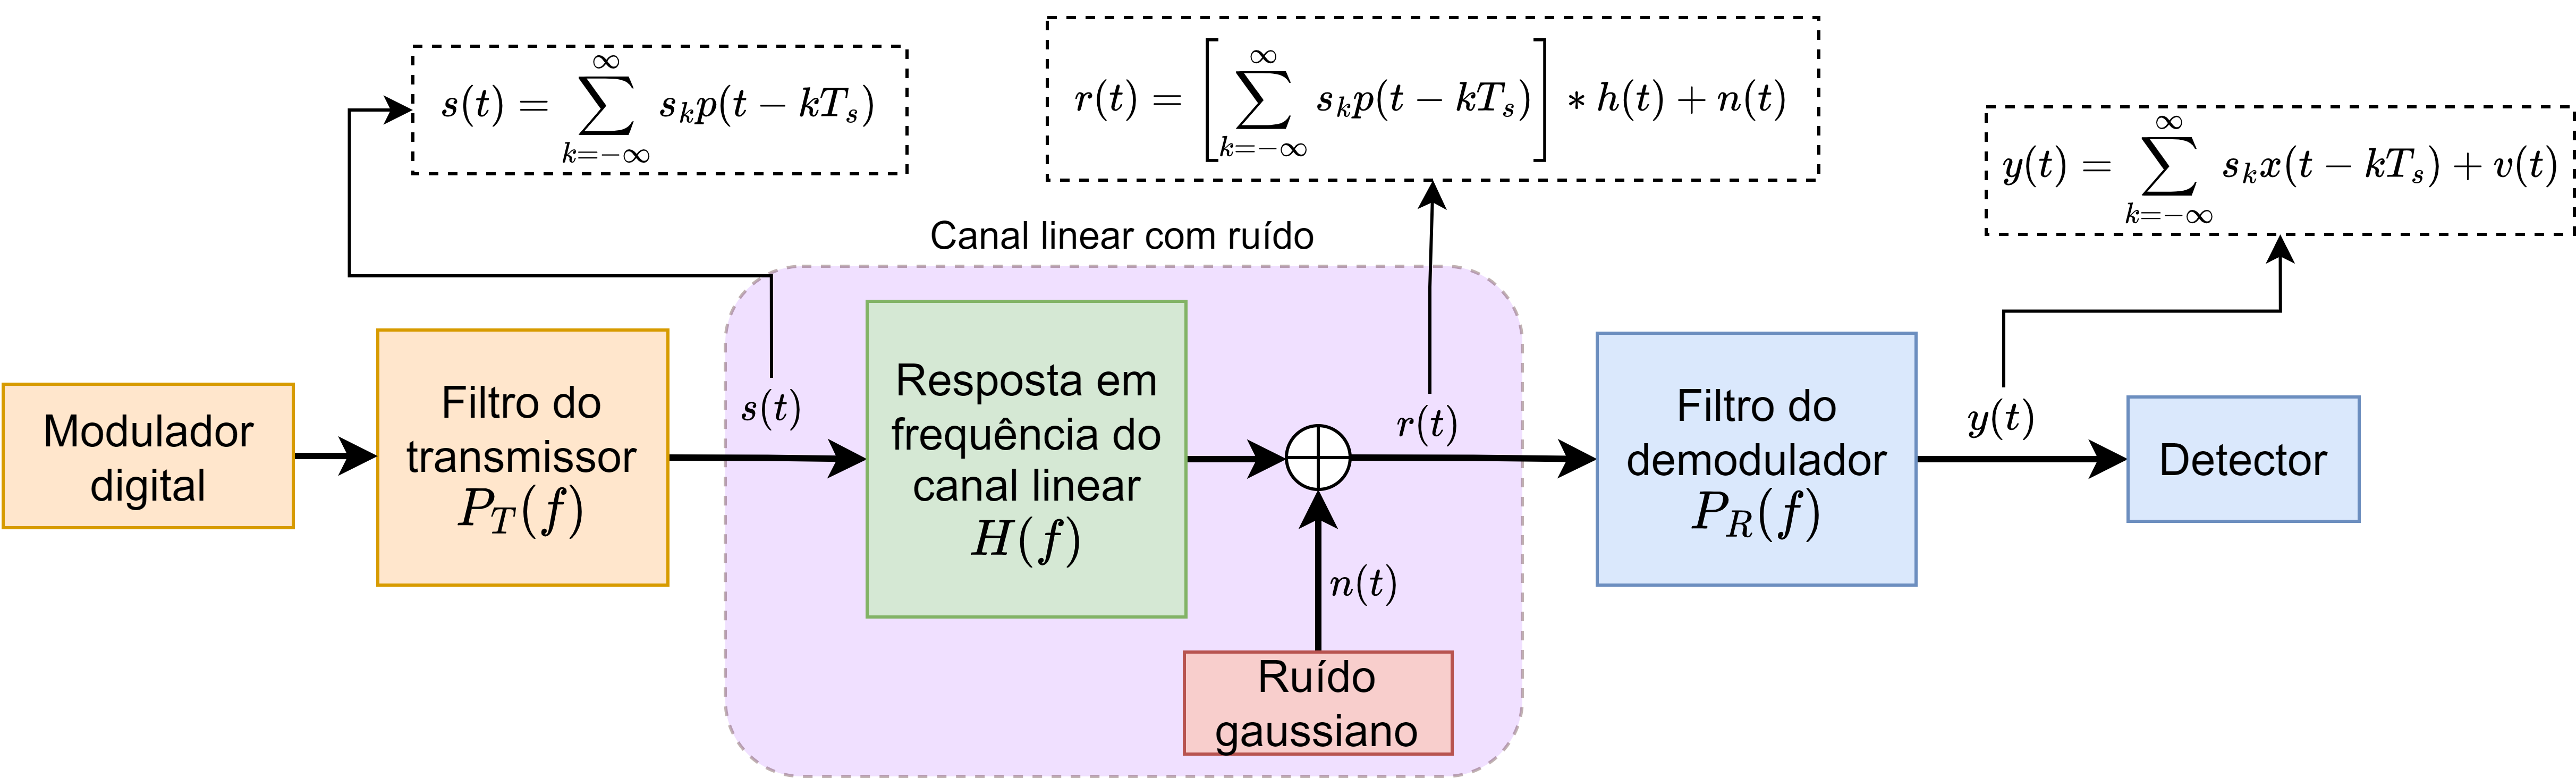
\includegraphics{figuras/Fig14.png}

Fig.2: Esquemático de um sistema de transmissão digital via canal linear
e AWGN.

Desse modo, o sinal \(r(t)\) que chega a entrada do receptor pode ser
representado por

\[
\begin{align}
r(t) & =\left[\sum_{k=-\infty}^{\infty} s_k p\left(t-k T_s\right)\right] \ast h(t) + n(t)\nonumber \\
& =\sum_{k=-\infty}^{\infty} s_k p(t)\ast \delta\left(t-k T_s\right) \ast h(t) + n(t)\nonumber \\
& =\sum_{k=-\infty}^{\infty} s_k p(t)\ast h(t)\ast\delta\left(t-k T_s\right)  + n(t)\nonumber \\
& =\sum_{k=-\infty}^{\infty} s_k g(t)\ast\delta\left(t-k T_s\right)  + n(t)\nonumber \\
& =\sum_{k=-\infty}^{\infty} s_k g\left(t-k T_s\right)  + n(t) \label{ch_model_1}\\
\end{align}
\]

em que \(g(t)\) é o pulso resultante da convolução de \(p(t)\) com a
resposta ao impulso do canal \(h(t)\).

\begin{block}{Interferência intersimbólica (ISI)}
\phantomsection\label{interferuxeancia-intersimbuxf3lica-isi}
Assuma que no receptor o sinal \(r(t)\) é filtrado e amostrado nos
instantes \(t=qT_s + \tau_{0}, q=0, 1, \ldots\). Seja a saída do filtro
do receptor dada por

\begin{equation}
y(t)=\sum_{k=-\infty}^{\infty} s_k x(t-kT_s) + v(t)
\end{equation}

temos

\begin{equation}
y\left(q T_s+\tau_0\right) \equiv y_q=\sum_{k=-\infty}^{\infty} s_k x\left(qT_s- kT_s+\tau_0\right) + v\left(qT_s+\tau_0\right)
\end{equation}

em que \(\tau_{0}\) é o atraso de propagação do sinal pelo canal.
Considerando apenas a representação discreta do sinal, temos

\[
\begin{align}
y_q&=\sum_{k=-\infty}^{\infty} s_k x_{q-k}+v_q, \quad q=0,1, \ldots.\nonumber\\
&= x_0\left(s_q+\frac{1}{x_0} \sum_{\substack{k=-\infty \\ k \neq q}}^{\infty} s_k x_{q-k}\right)+v_q, \quad q=0,1, \ldots
\end{align}
\]

em que \(x_0\) é um fator de escala arbitrário que pode ser considerado
igual à unidade por conveniência, de modo que

\begin{equation}\label{ISI_eq1}
y_q=s_q + \sum_{\substack{k=-\infty \\ k \neq q}}^{\infty} s_k x_{q-k} + v_q, \quad q=0,1, \ldots
\end{equation}

Em (\(\ref{ISI_eq1}\)), temos que \(s_q\) é o símbolo transmitido no
intervalo de sinalização \(q\). Já o termo
\(\sum_{\substack{k=-\infty \\ k \neq q}}^{\infty} s_k x_{q-k}\)
representa a interferência causada em \(s_q\) pelos demais símbolos
transmitidos, denominada \textbf{interferência intersimbólica}
(\emph{intersymbol interference} - ISI). Por fim, \(v_q\) é uma variável
aleatória representado o ruído AWGN no instante de sinalização \(q\).

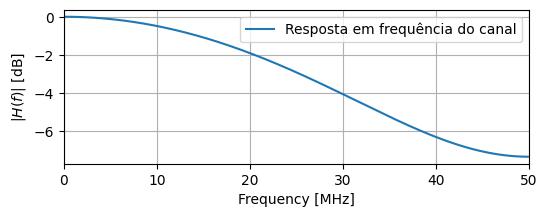
\includegraphics{figuras/nb3_out_0.png}

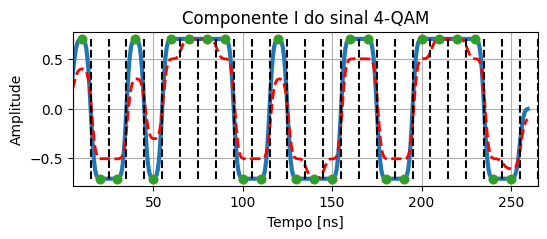
\includegraphics{figuras/nb3_out_1.png}

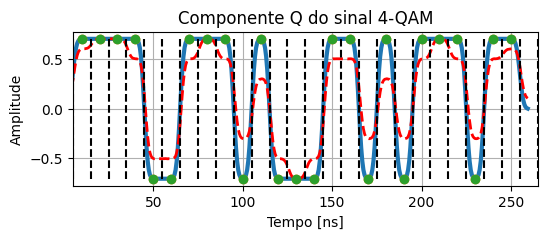
\includegraphics{figuras/nb3_out_2.png}

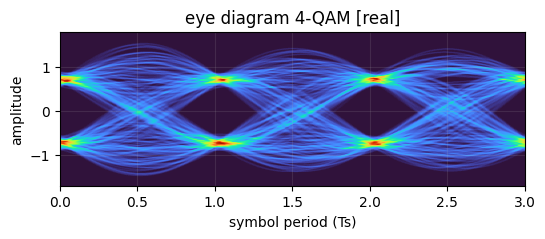
\includegraphics{figuras/nb3_out_3.png}

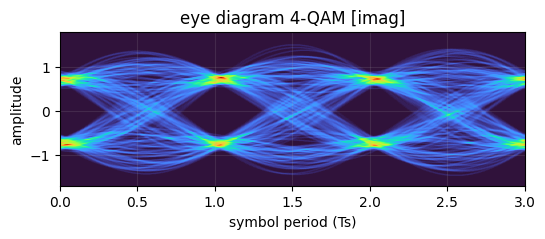
\includegraphics{figuras/nb3_out_4.png}

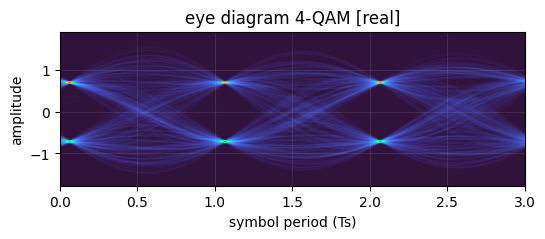
\includegraphics{figuras/nb3_out_5.png}

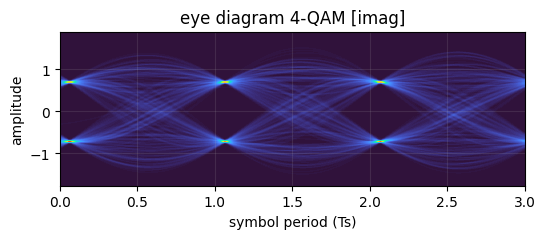
\includegraphics{figuras/nb3_out_6.png}

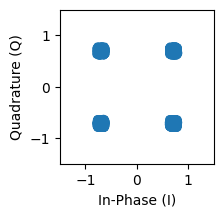
\includegraphics{figuras/nb3_out_7.png}

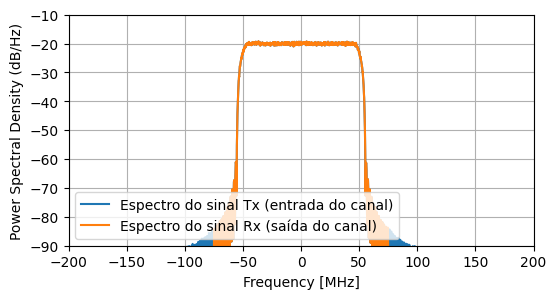
\includegraphics{figuras/nb3_out_8.png}
\end{block}

\begin{block}{Critério de Nyquist para ausência de interferência
intersimbólica}
\phantomsection\label{crituxe9rio-de-nyquist-para-ausuxeancia-de-interferuxeancia-intersimbuxf3lica}
Considere que a resposta em frequência \(H(f)\) é ideal e limitada em
banda, de maneira que

\begin{equation}
H(f) = \begin{cases}1, & |f|<B \\ 0, & \text { caso contrário.}\end{cases}.
\end{equation}

Logo, assumindo que o receptor aplica um filtro casado ao pulso \(p(t)\)
transmitido, temos que \(X(f) = |P(f)|^2\), em que

\begin{equation}
x(t) = \int_{-B}^{B}X(f)e^{2\pi f t} df.
\end{equation}

Desejamos encontrar as condições que \(p(t)\) deve atender e, por
consequência, \(x(t)\), para que a interferência intersimbólica seja
nula. Sabemos que

\begin{equation}\label{ISI_eq2}
y_q=s_q + \sum_{\substack{k=-\infty \\ k \neq q}}^{\infty} s_k x_{q-k} + v_q, \quad q=0,1, \ldots,
\end{equation}

o que implica que a condição para ausência de ISI é dada por

\begin{equation}\label{isi_x}
x(t=n T_s) \equiv x_n= \begin{cases}1, & n=0 \\ 0, & n \neq 0\end{cases}
\end{equation}

Esta condição é conhecida como critério de Nyquist para ausência de
interferência intersimbólica.

\textbf{Teorema (Critério de Nyquist)}: uma condição necessária e
suficiente para a ausência de interferência intersimbólica, ou seja,
para \(x(t)\) satisfazer (\(\ref{isi_x}\)) é que sua transformada de
Fourier \(X(f)\) satisfaça

\[
\sum_{m=-\infty}^{\infty} X(f+m R_s)=T_s.
\]

Prova:

Considere a transformada inversa de Fourier
\(x(t) = \mathcal{F}^{-1}\{X(f)\}\):

\begin{equation}
x(t)=\int_{-\infty}^{\infty} X(f) e^{j 2 \pi f t} d f
\end{equation}

As amostras do pulso \(x(t)\) são tomadas ao final de cada intervalo de
sinalização, nos instantes \(t=kT_s\). Desse modo

\begin{equation}
x(kT_s) =\int_{-\infty}^{\infty} X(f) e^{j 2 \pi f k T_s} d f.
\end{equation}

A taxa de sinalização, ou taxa de símbolos, \(R_s\) é dada por
\(R_s = 1/T_s\), de modo que

\[
\begin{align}
x(kT_s) & =\sum_{m=-\infty}^{\infty} \int_{(2 m-1) R_s/2}^{(2 m+1) R_s/2} X(f) e^{j 2 \pi f kT_s} d f\nonumber \\
& =\sum_{m=-\infty}^{\infty} \int_{-R_s/2}^{R_s/2} X(f+ m R_s) e^{j 2 \pi f kT_s} d f \nonumber\\
& =\int_{-R_s/2}^{R_s/2}\left[\sum_{m=-\infty}^{\infty} X(f+m R_s)\right] e^{j 2 \pi f kT_s} d f \nonumber\\
& =\int_{-R_s/2}^{R_s/2} B(f) e^{j 2 \pi f kT_s} d f\label{nyq_1}
\end{align}
\]

em que a função \(B(f)\) é dada por

\begin{equation}
B(f)=\sum_{m=-\infty}^{\infty} X(f+mR_s).
\end{equation}

Como \(B(f)\) é periódica em \(f\) com período \(R_s\), esta admite
representação em termos de uma série de Fourier

\[
\begin{align}
B(f)&=\sum_{k=-\infty}^{\infty} b_k e^{j 2 \pi k f T_s} \nonumber \\
b_k&=\frac{1}{R_s} \int_{-R_s / 2}^{R_s/ 2} B(f) e^{-\frac{j2 \pi k f}{R_s}} d f = T_s \int_{-R_s / 2}^{R_s/ 2} B(f) e^{-j2 \pi k f T_s} d f \label{nyq_2}
\end{align}
\]

Logo, comparando (\(\ref{nyq_1}\)) e (\(\ref{nyq_2}\)), temos que

\begin{equation}
b_k=T_s x(-k T_s).
\end{equation}

Desse modo, na ausência de ISI, os coeficientes \(b_k\) devem ser dados
por \begin{equation}\label{fourier_coeffs}
b_k=\begin{cases}T_s, & k=0 \\ 0, & k \neq 0\end{cases}.
\end{equation}

o que implica em

\[
\begin{align}
B(f)&=T_s\\
\sum_{m=-\infty}^{\infty} X(f+m R_s)&=T_s.
\end{align}
\]

Supondo que o canal tem banda \(B\), teremos então três casos

\begin{enumerate}
\item
  Se \(R_s > 2B\), as cópias de \(X(f)\) espaçadas de \(R_s\) no domínio
  da frequência não se sobrepõem, de modo que não há nenhuma escolha
  possível de \(x(t)\) que permita que
  \(\sum_{m=-\infty}^{\infty} X(f+m R_s)\) seja uma função constante.
  Como consequência, não existe nenhuma função \(x(t)\) que permita a
  transmissão livre de ISI.
\item
  Se \(R_s = 2B\), o somatório \(\sum_{m=-\infty}^{\infty} X(f+m R_s)\)
  será uma constante apenas se \(X(f)\) for uma função porta \begin{equation}
  X(f)= \begin{cases}T_s & |f|<B \\ 0, & \text { c.c. }\end{cases}
  \end{equation}
\end{enumerate}

ou seja, se \(x(t)\) for uma função sinc

\begin{equation}
x(t)=\operatorname{sinc}\left(\frac{t}{T_s}\right).
\end{equation}

\begin{enumerate}
\setcounter{enumi}{2}
\tightlist
\item
  Se \(R_s < 2B\), os temos do somatório
  \(\sum_{m=-\infty}^{\infty} X(f+m R_s)\) se sobrepõem, de modo que
  existirão diversas escolhas de \(x(t)\) que o mesmo seja constante.
\end{enumerate}
\end{block}

\begin{block}{Família de pulsos cosseno levantado (\emph{raised
cosine})}
\phantomsection\label{famuxedlia-de-pulsos-cosseno-levantado-raised-cosine}
Um conjunto de pulsos que atendem ao critério de Nyquist de ISI nula
correponde à família de pulsos cosseno levantado, que pode ser definida
no domínio da frequência como \begin{equation}
X_{r c}(f)= \begin{cases}T_s, & 0 \leq|f| \leq(1-\alpha) / 2 T_s \\ \frac{T_s}{2}\left[1+\cos \frac{\pi T_s}{\alpha}\left(|f|-\frac{1-\alpha}{2 T_s}\right)\right], & \frac{1-\alpha}{2 T_s} \leq|f| \leq \frac{1+\alpha}{2 T_s} \\ 0, & |f|>\frac{1+\alpha}{2 T_s}\end{cases}
\end{equation} e no domínio do tempo como \[
\begin{align}
x(t) & =\frac{\operatorname{sen} (\pi t / T_s)}{\pi t / T_s} \frac{\cos (\pi \alpha t / T_s)}{1-4 \alpha^2 t^2 / T_s^2}\nonumber \\
& =\operatorname{sinc}(t / T_s)\frac{\cos (\pi \alpha t / T_s)}{1-4 \alpha^2 t^2 / T_s^2},
\end{align}
\]

em que \(0<\alpha<1\) é denominado de parâmetro de \emph{rolloff} ou
\emph{excesso de banda}.

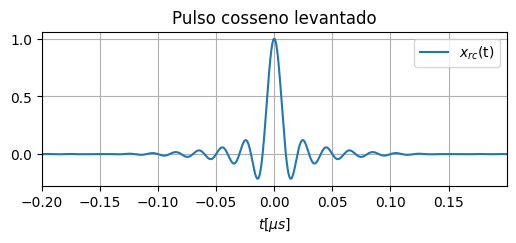
\includegraphics{figuras/nb3_out_9.png}

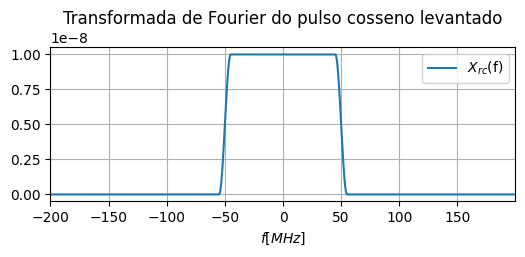
\includegraphics{figuras/nb3_out_10.png}

Duas vantagens importantes:

\begin{enumerate}
\item
  Devido às características suaves de transição de \(x_{rc}(t)\) estes
  pulsos podem ser implementados na prática por filtros lineares
  formatadores de pulso.
\item
  As bordas laterais dos pulsos \(x_{rc}(t)\) convergem para 0 a uma
  taxa proporcional a \(1/t^3\), para \(\alpha>0\), diferentemente da
  função \(\operatorname{sinc}(t)\), que convege a \(1/t\). Essa
  proprieadade permite que pequenos desvios do instante de amostragem
  ótimo façam com que a ISI convirja para um valor finito no caso do
  pulso \(x_{rc}(t)\), enquanto a mesma diverge no caso de pulsos
  \(\operatorname{sinc}(t)\). Assim, pulsos \(x_{rc}(t)\) são em geral
  mais robustos à erros de sincronização do que pulsos
  \(\operatorname{sinc}(t)\).
\item
  A complexidade do processamento requerido para a implementação de
  \(x_{rc}(t)\) pode ser dividida entre transmissor e receptor.
  Considerando a situação ideal em que \begin{equation}\nonumber
  H(f) = \begin{cases}1, & |f|<B \\ 0, & \text { caso contrário.}\end{cases}
  \end{equation}Sejam \(P_T(f)\) e \(P_R(f) = P_T^*(f)\) os filtro formatador de
  pulso do transmissor e o filtro casado correspondente no receptor,
  respectivamente, temos que\[
  \begin{align}
  P_T(f)H(f)P_R(f) &= X_{rc}(f)\nonumber\\
  P_T(f)P_R(f) &= X_{rc}(f)\nonumber\\
  |P_T(f)|^2 &= X_{rc}(f)\nonumber\\
  \end{align}
  \] ou seja, \(X_{rc}(f)\) pode ser alcançada fazendo-se
  \(P_T(f) = P_R^*(f) = \sqrt{X_{rc}(f)} = P_{rrc}(f)\). O pulso cujo
  espectro é dado por \(P_{rrc}(f) = \sqrt{X_{rc}(f)}\) é conhecido como
  raiz do cosseno levantado (\emph{root raised cosine} - RRC) e é
  definido no domínio do tempo por
\end{enumerate}

\[
p_{rrc}(t)= \begin{cases}\frac{1}{T_s}\left(1+\alpha\left(\frac{4}{\pi}-1\right)\right), & t=0 \\ \frac{\alpha}{T_s \sqrt{2}}\left[\left(1+\frac{2}{\pi}\right) \sin \left(\frac{\pi}{4 \alpha}\right)+\left(1-\frac{2}{\pi}\right) \cos \left(\frac{\pi}{4 \alpha}\right)\right], & t= \pm \frac{T_s}{4 \alpha} \\ \frac{1}{T_s} \frac{\sin \left[\pi \frac{t}{T_s}(1-\alpha)\right]+4 \alpha \frac{t}{T_s} \cos \left[\pi \frac{t}{T_s}(1+\alpha)\right]}{\pi \frac{t}{T_s}\left[1-\left(4 \alpha \frac{t}{T_s}\right)^2\right]}, & \text { caso contrário.}\end{cases}
\]
\end{block}

\begin{block}{Transmissão de sinais com \emph{resposta parcial}}
\phantomsection\label{transmissuxe3o-de-sinais-com-resposta-parcial}
Para efeitos práticos, o critério de Nyquist nos indica que é possível
projetar formas de pulso para eliminar a presença de ISI no receptor,
desde que a taxa de sinalização \(R_s\) da transmissão em
símbolos/segundo seja tal que \(R_s < 2B\), em que \(B\) é a banda do
canal de comunicações em Hz.

Entretanto, transmitir a uma taxa de \(R_s = 2B\) sem ter que recorrer à
utilização de pulsos \(\operatorname{sinc}(t)\) ainda será possível,
desde que uma determinada quantidade controlada de ISI possa ser
tolerada no receptor. Por exemplo, suponha que

\[
x(k T_s)= \begin{cases} 1, & k=0,1 \\ 0, & \text { caso contrário. }\end{cases}
\]

e então, os coeficientes em (\(\ref{fourier_coeffs}\)) serão dados por

\[
b_k= \begin{cases}T_s & k=0,-1 \\ 0 & \text { caso contrário, }\end{cases}
\]

de maneira que
\(B(f)=T_s + T_s e^{j 2 \pi f T_s} = T_s\left(1 + e^{j 2 \pi f T_s}\right)\)

Se \(R_s > 2B\), o problema continua sem solução. Já no caso de
\(R_s=2B\), \(B(f)\) pode ser alcançado se fizermos

\[
\begin{align} 
X(f) & = \begin{cases}\frac{1}{2 B}\left(1+e^{-j \pi f / B}\right) & |f|<B \\ 0 & \text { caso contrário} \end{cases}\nonumber \\ 
& = \begin{cases}\frac{1}{B} e^{-j \pi f / 2 B} \cos\left( \frac{\pi f}{2 B}\right) & |f|<B \\ 0 & \text { caso contrário}\end{cases}. \nonumber\end{align}
\]
\end{block}

\begin{block}{Visualizando \(X(f)\) e \(B(f)\)}
\phantomsection\label{visualizando-xf-e-bf}
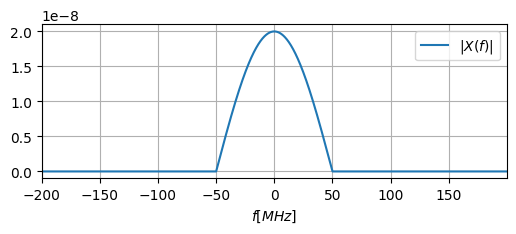
\includegraphics{figuras/nb3_out_11.png}

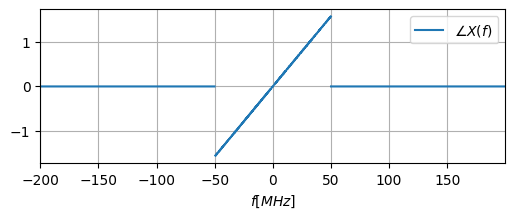
\includegraphics{figuras/nb3_out_12.png}

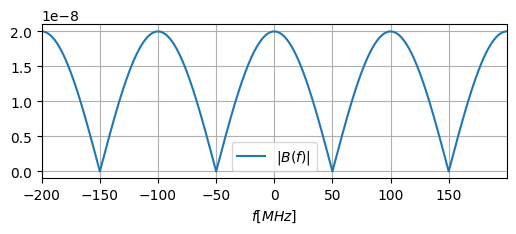
\includegraphics{figuras/nb3_out_13.png}

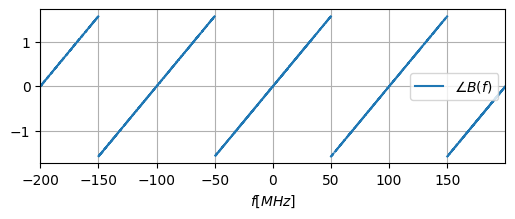
\includegraphics{figuras/nb3_out_14.png}

No domínio do tempo, o pulso associado a \(X(f)\) é dado por

\[
x(t)=\operatorname{sinc}(2 \pi B t)+\operatorname{sinc}\left(2\pi B(t-T_s)\right)
\]

que é conhecido como \emph{pulso duobinário}.

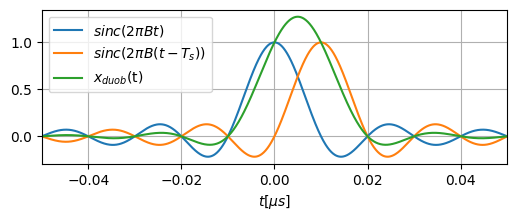
\includegraphics{figuras/nb3_out_15.png}

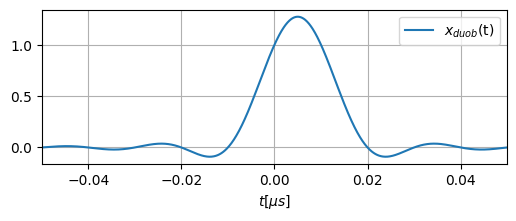
\includegraphics{figuras/nb3_out_16.png}

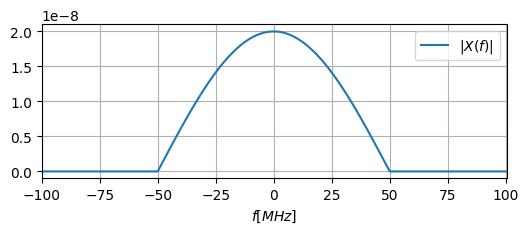
\includegraphics{figuras/nb3_out_17.png}

Outra possibilidade é fazer

\[
x(kT_s)= \begin{cases} 1, & k=-1 \\ -1, & k =1\\ 0, & \text { caso contrário. }\end{cases}
\]

que resultará no pulso

\[
x(t)=\operatorname{sinc}\left[2\pi B(t+T_s)\right]-\operatorname{sinc}\left[2\pi B(t-T_s)\right]
\]

cujo espectro é dado por

\[
X(f)= \begin{cases}\frac{1}{2 B}\left(e^{i \pi f / B}-e^{-j \pi f/ B}\right)=\frac{j}{B} \sin \left(\frac{\pi f}{B}\right) & |f|\leqslant B \\ 0 & |f| > B\end{cases}
\]

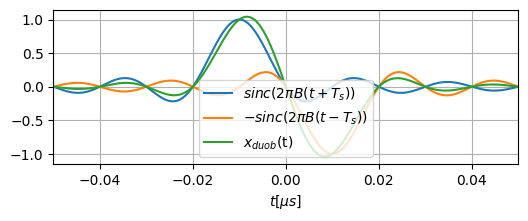
\includegraphics{figuras/nb3_out_18.png}

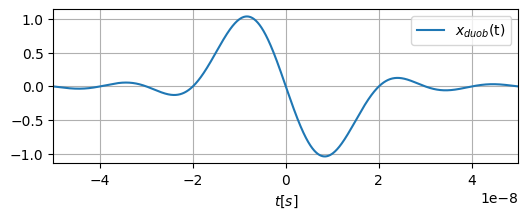
\includegraphics{figuras/nb3_out_19.png}

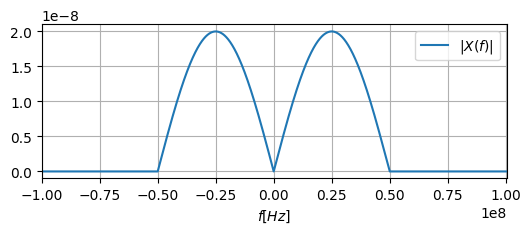
\includegraphics{figuras/nb3_out_20.png}

De maneira geral, os pulsos pertencentes ao conjunto de sinais limitados
em banda que são definidos como

\[
x(t)=\sum_{n=-\infty}^{\infty} x\left(\frac{n}{2 B}\right) \operatorname{sinc}\left[2 \pi B\left(t-\frac{n}{2 B}\right)\right]
\]

e com espectro correspondente

\[
X(f)= \begin{cases}\frac{1}{2 B} \sum_{n=-\infty}^{\infty} x\left(\frac{n}{2 B}\right) e^{-j n \pi f / B} & |f| \leqslant B \\ 0, & \text{caso contrário.}\end{cases}
\]

são denominados pulsos ou sinais de \emph{resposta parcial}. A
utilização de tais pulsos na transmissão significa que há uma adição
controlada de ISI por meio da introdução de duas ou mais amostras
não-nulas \(x\left(\frac{n}{2 B}\right)\). Tais pulsos permitem a taxa
de sinalização da transmissão seja igual a taxa de Nyquist, ou seja,
\(R_s = 2B\).
\end{block}

\begin{block}{Exemplos:}
\phantomsection\label{exemplos}
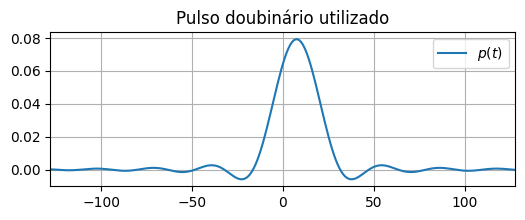
\includegraphics{figuras/nb3_out_21.png}

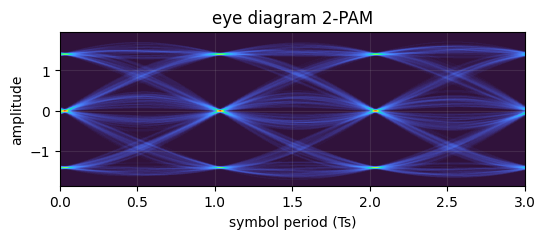
\includegraphics{figuras/nb3_out_22.png}

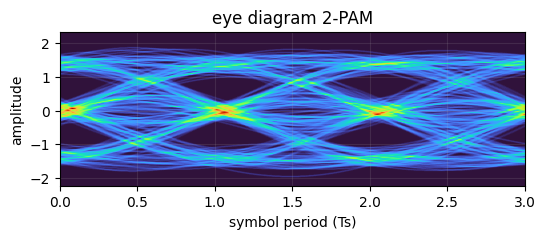
\includegraphics{figuras/nb3_out_23.png}

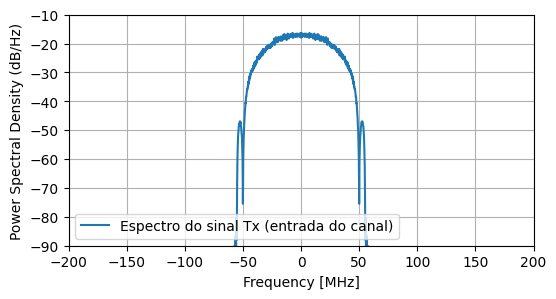
\includegraphics{figuras/nb3_out_24.png}

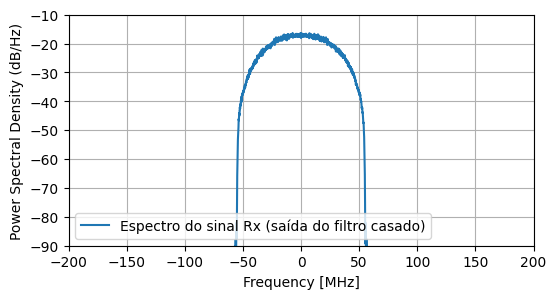
\includegraphics{figuras/nb3_out_25.png}

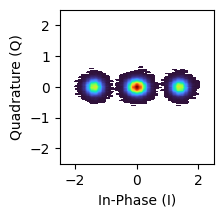
\includegraphics{figuras/nb3_out_26.png}
\end{block}

\begin{block}{Detecção símbolo-a-símbolo de sinais com ISI controlada}
\phantomsection\label{detecuxe7uxe3o-suxedmbolo-a-suxedmbolo-de-sinais-com-isi-controlada}
Considere uma transmissão duobinária tal que a amostra \(y_k\) capturada
em cada instante de sinalização \(t=kT_s\) seja dada por

\[
y_k = r_k + v_k = a_k + a_{k-1} + v_k
\]

em que \{\(a_k\)\} é a sequência de amplitudes transmitidas e
\{\(v_k\)\} a sequência de amostras de ruído aditivo gaussiano.
Considere que \(a_k=\pm 1\), com a mesma probabilidade, de modo que
\(r_k=-2,0,2\) com probabilidades \(1/4\), \(1/2\) e \(1/4\).

Note que, se \(a_{k-1}\) for conhecido, o receptor pode simplesmente
subtrair seu valor de \(r_k\), de modo a eliminar o efeito da ISI.
Entretanto, se o receptor cometeu um erro na detecção de \(a_{k-1}\), a
subtração tenderá a não eliminarar a ISI em \(r_k\), podendo até mesmo
amplificar o efeito da ISI. Tal fenômeno é conhecido como
\emph{propagação de erros}.

A propagação de erros pode ser evitada utilizando-se uma pré-codificação
na sequência de bits a ser transmitida.

Considere que a partir de uma sequência de bits \(b_k\), uma nova
sequência \(c_k\) seja gerada fazendo

\begin{equation}\label{precod}
c_k = b_k \ominus c_{k-1}, \quad k = 1, 2, \ldots
\end{equation}

em que \(\ominus\) representa a operação de subtração módulo-2 (que é
idêntica à operação \(\oplus\) adição módulo-2, ou XOR).

Considerando que a modulação utilizada é a 2-PAM antipodal, temos que a
sequência correspondente de amplitudes da modulação é dada por

\[
a_k = 2c_k -1.
\]

Consequentemente, a sequência de amplitudes do sinal \emph{duobinário}
produzido a partir de \(a_k\) é dada por

\[
r_k = a_k + a_{k-1}.
\]

Temos então que

\begin{align}
r_k &= a_k + a_{k-1}\nonumber\\
&= (2c_k -1) + (2c_{k-1} -1)\nonumber\\
&= 2(c_k + c_{k-1}-1)\nonumber\\
\end{align}

ou seja,

\[
c_k + c_{k-1} = \frac{r_k}{2} + 1
\]

De (\(\ref{precod}\)) temos que \(c_k \oplus c_{k-1} = b_k\), de modo
que

\[
b_k=\frac{r_k}{2} + 1 (\bmod 2)
\]

A regra de decisão no receptor torna-se, então

\[
b_k = \begin{cases}0, & r_k = +2, -2\\
1, & r_k = 0.
\end{cases}
\]

Com a presença de ruído, as amostras observadas pelo receptor são dadas
por \(y_k = r_k + v_k\), de modo que a decisão pode ser tomada baseada
na comparação do sinal recebido com dois limiares de decisão
posicionados em +1 e -1, ou seja

\[
b_k= \begin{cases}1, & \text { se }-1<y_k<1 \\ 0, & \text { se }\left|y_k\right| \geq 1\end{cases}
\]

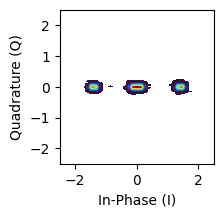
\includegraphics{figuras/nb3_out_27.png}

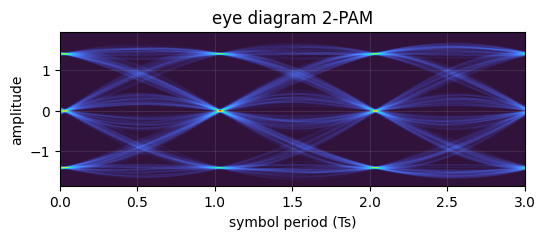
\includegraphics{figuras/nb3_out_28.png}

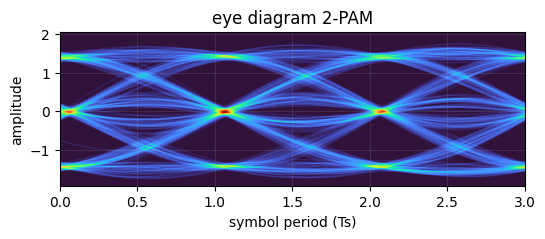
\includegraphics{figuras/nb3_out_29.png}

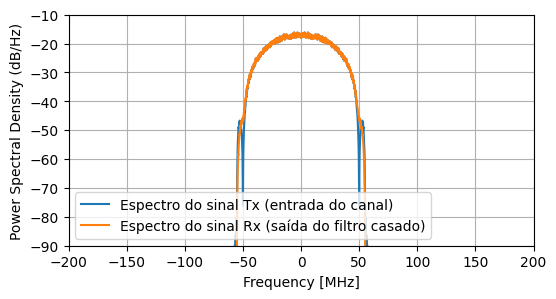
\includegraphics{figuras/nb3_out_30.png}
\end{block}
\end{frame}

\begin{frame}{Detecção de sequências por máxima verossimilhança}
\phantomsection\label{detecuxe7uxe3o-de-sequuxeancias-por-muxe1xima-verossimilhanuxe7a}
Considere o caso em que sequência de sinais recebidos não está sujeita a
nenhum efeito de memória, ou seja, o vetor \(\mathbf{r}_k\) observado no
intervalo de sinalização \(k\) é \emph{estatisticamente independente}
dos vetores
\(\left\lbrace \mathbf{r}_{k'} \right\rbrace_{k'=-\infty}^{\infty}\) e
\(k' \neq k\), observados nos demais intervalos de sinalização. Neste
caso, o detector que opera \emph{símbolo-a-símbolo}, ou seja, que decide
utilizando apenas a informação \(P(\mathbf{s}_m|\mathbf{r}_k)\) presente
no intervalo de sinalização \(k\) é o detector ótimo no sentido de
minimização da probabilidade de erro.

Entretanto, na presença de memórioa, ou seja, caso exista
\emph{dependência estatística} entre a sequência de sinais
\(\left\lbrace \mathbf{r}_{k} \right\rbrace_{k=-\infty}^{\infty}\), o
detector ótimo para o sinal recebido no intervalo de sinalização \(k\)
deverá levar em conta não apenas este intervalo de sinalização, mas uma
sequência de intervalos de sinalização consecutivos.

Como exemplo, considere o caso da transmissão duobinária 2-PAM. Seja
\(L\) o intervalo de mémoria, em intervalos de sinalização, presente na
transmissão, para um sinal duobinário temos que \(L=1\).

\[
\begin{aligned}
\begin{array}{|c|c|c|c|}
  \hline
  a_{k-1} & a_{k} & r_{k} = a_k + a_{k-1}  \\
  \hline
  -1 & -1 & -2 \\
  \hline
  1 & -1 & 0  \\
  \hline
  -1 & 1 & 0 \\
  \hline
  1 & 1 & 2 \\
  \hline
\end{array}
\end{aligned}
\]

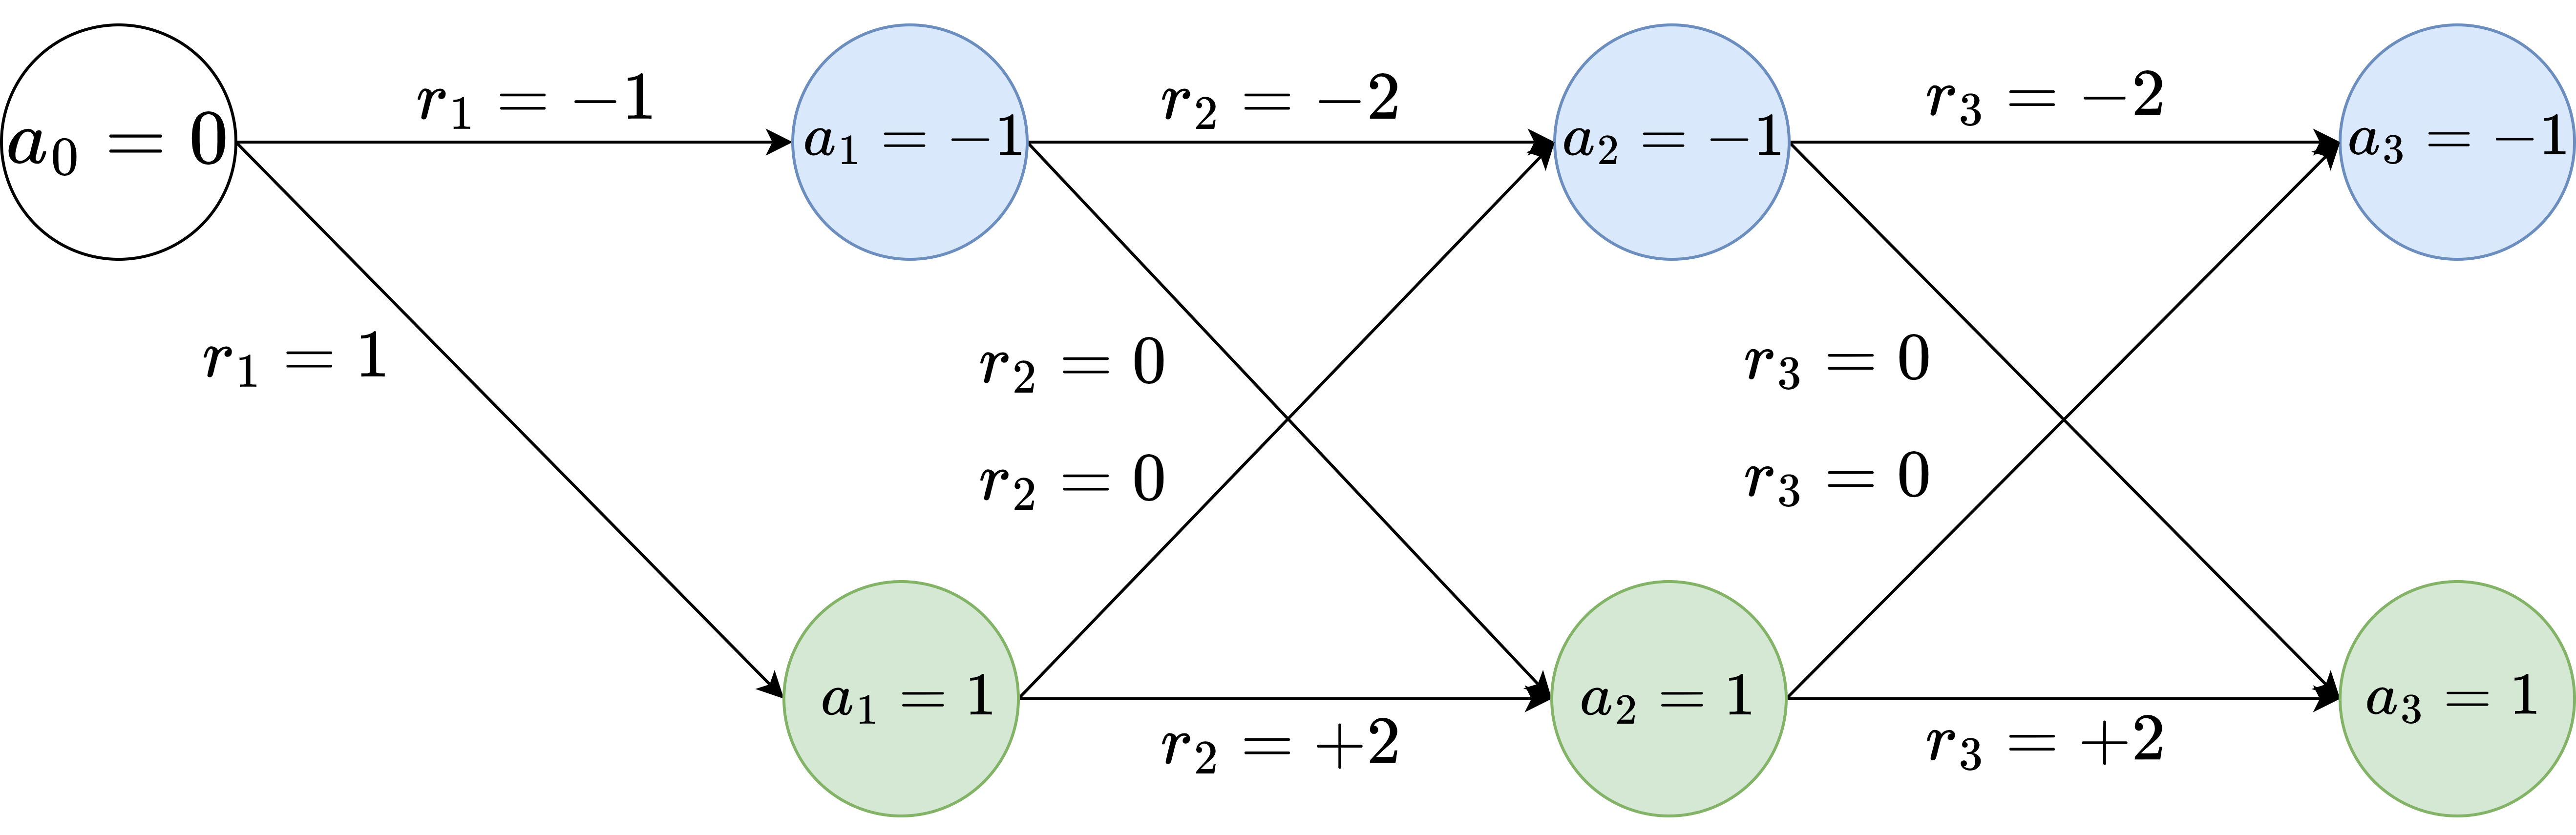
\includegraphics{figuras/Fig13.png}

Fig.10: Treliça representando a evolução de estados da modulação 2-PAM
duobinário.

Considere um vetor \(\boldsymbol{y}\) composto pela sequência de
amostras da saída do filtro do receptor sobre \(N\) intervalos de
sinalização \(\boldsymbol{y} = [y_1, y_2, \dots, y_N]^T\). Temos que

\[\boldsymbol{y} = \boldsymbol{r} + \boldsymbol{v}\]

em que \(\boldsymbol{r} = [r_1, r_2, \dots, r_N]^T\) é a sequência de
amplitudes do sinal duobinário livres de ruído,
\(\boldsymbol{v} = [v_1, v_2, \dots, v_N]^T\) é a sequência de amostras
de ruído gaussiano,
i.e.~\(\boldsymbol{v}\sim \mathcal{N}(\mathbf{0}, \Sigma_v)\).

Seja \(\boldsymbol{a} = [a_1, a_2, \dots, a_N]^T\) a sequência de
amplitudes binárias transmitidas, a fdp condicional
\(p(\boldsymbol{y}|\boldsymbol{a})\) pode ser escrita como

\[
p(\boldsymbol{y}|\boldsymbol{a}) = \frac{1}{(2\pi |\Sigma_v|)^{N/2}} \exp \left[-\frac{1}{2} (\boldsymbol{y}-\boldsymbol{r})^T \Sigma_v^{-1} (\boldsymbol{y}-\boldsymbol{r}) \right].
\]

Desse modo, temos que a probabilidade da sequência \(\boldsymbol{a}\)
ter sido transmitida condicionada à sequência de observações
\(\boldsymbol{y}\) pode ser escrita como \[
P(\boldsymbol{a}|\boldsymbol{y}) = \frac{p(\boldsymbol{y}|\boldsymbol{a})P(\boldsymbol{a})}{p(\boldsymbol{y})} \propto p(\boldsymbol{y}|\boldsymbol{a})P(\boldsymbol{a})
\]

Assumindo que o detector decidirá por uma sequência
\(\boldsymbol{\hat{a}}\), a decisão ótima será tal que

\[\boldsymbol{\hat{a}} = \underset{\boldsymbol{a}}{\operatorname{argmax}} p(\boldsymbol{y}|\boldsymbol{a})P(\boldsymbol{a})\].

correspondendo ao critério MAP.

Considerando que todas as sequências são equiprováveis

\[
P(\boldsymbol{a}|\boldsymbol{y}) \propto p(\boldsymbol{y}|\boldsymbol{a})
\]

de modo que

\[\boldsymbol{\hat{a}} = \underset{\boldsymbol{a}}{\operatorname{argmax}} p(\boldsymbol{y}|\boldsymbol{a})\],

que corresponde ao critério de decisão ML.

\[
\ln p(\boldsymbol{y}|\boldsymbol{a}) = -\frac{N}{2}\ln(2\pi |\Sigma_v|) -\frac{1}{2} (\boldsymbol{y}-\boldsymbol{r})^T \Sigma_v^{-1} (\boldsymbol{y}-\boldsymbol{r})
\]

Maximizar \(\ln p(\boldsymbol{y}|\boldsymbol{a})\) equivale a encontrar
a sequência \(\boldsymbol{a}\) que minimiza
\((\boldsymbol{y}-\boldsymbol{r})^T \Sigma_v^{-1} (\boldsymbol{y}-\boldsymbol{r})\)

\[\boldsymbol{\hat{a}} = \underset{\boldsymbol{a}}{\operatorname{argmin}} (\boldsymbol{y}-\boldsymbol{r})^T \Sigma_v^{-1} (\boldsymbol{y}-\boldsymbol{r})\],

como \(r_k =x_0a_k + x_1a_{k-1} + \dots =  \sum_{q=0}^{L}x_qa_{k-q}\)

\[\boldsymbol{\hat{a}} = \underset{\boldsymbol{a}}{\operatorname{argmin}} \left[ \sum_{m=1}^{N}\left(y_m - \sum_{q=0}^{L}x_qa_{m-q}\right)^2\right]\],
\end{frame}

\begin{frame}{Referências}
\phantomsection\label{referuxeancias}
{[}1{]} J. G. Proakis, M. Salehi, Communication Systems Engineering, 2nd
Edition, Pearson, 2002.
\end{frame}

\end{document}
